\section{Introduction}

As outlined in the competition overview \cite{cassava-leaf-disease-classification}, cassava is an important crop in Africa, but its yields are significantly affected by diseases. The current disease monitoring primarily relies on visual inspection by agricultural experts, which is labor-intensive and costly. Thus, it is essential to identify common cassava diseases to address this issue. As illustrated in Fig.~\ref{CassavaDisease}, there are four main types of cassava diseases: Bacterial Blight, Brown Streak Disease, Green Mottle, and Mosaic Disease. Each disease displays distinct characteristics on the leaves, allowing for differentiation from healthy cassava leaves through image classifiers.

Bacterial Blight (Fig.~\ref{CassavaFigBac}) is characterized by dead leaf spots surrounded by yellow halos \cite{uwm2024BacterialBlight}. Brown Streak Disease (Fig.~\ref{CassavaFigBro}) presents as patches of yellow intermingled with the standard green color of the leaves \cite{patil2015cassava}. Green Mottle Disease (Fig.~\ref{CassavaFigGreen}) is identifiable by green spots on the leaves that appear as if they were painted on \cite{robson2024cassava}. Lastly, Mosaic Disease (Fig.~\ref{CassavaFigMos}) results in symptoms such as discoloration, with leaves showcasing variations of yellow, white, light, and dark shades \cite{chikoti2019cassava}.

\begin{figure}[htbp]
    \centering
    \begin{subfigure}{0.24\textwidth}
        \centering
        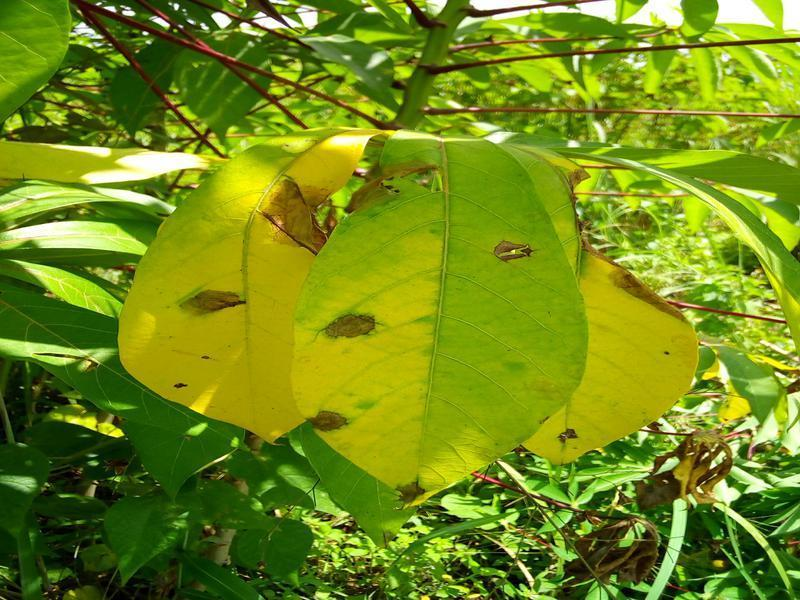
\includegraphics[width=\linewidth]{graphs/DiseaseImage/BacterialBlight.jpg}
        \caption{Bacterial Blight}
        \label{CassavaFigBac}
    \end{subfigure}
    \begin{subfigure}{0.24\textwidth}
        \centering
        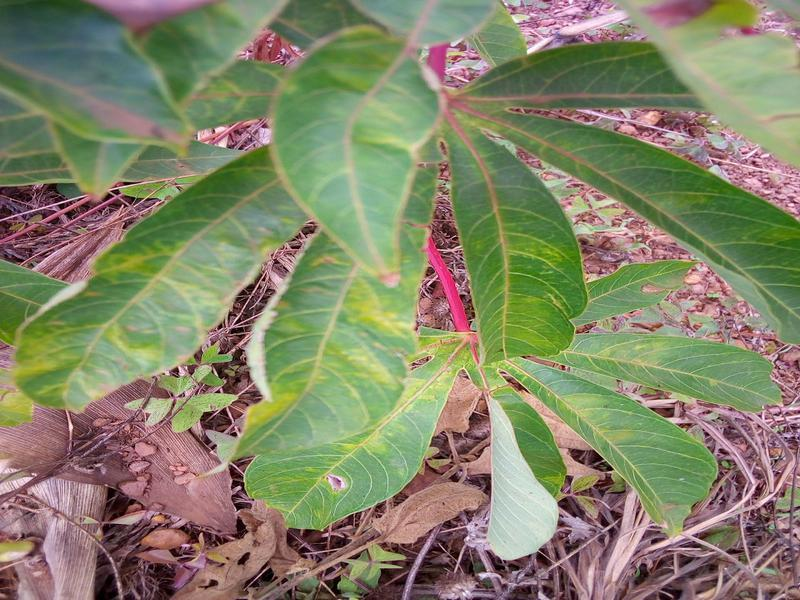
\includegraphics[width=\linewidth]{graphs/DiseaseImage/BrownStreak.jpg}
        \caption{Brown Streak}
        \label{CassavaFigBro}
    \end{subfigure}
    \begin{subfigure}{0.24\textwidth}
        \centering
        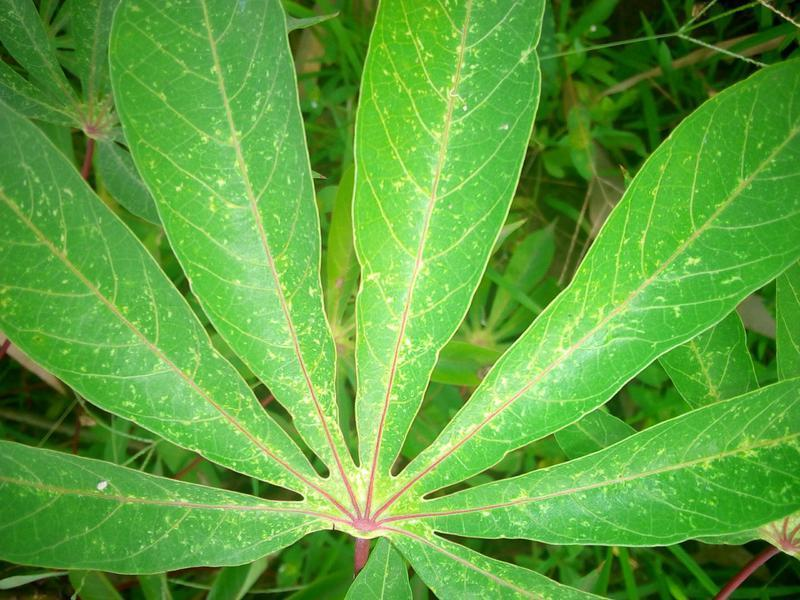
\includegraphics[width=\linewidth]{graphs/DiseaseImage/GreenMottle.jpg}
        \caption{Green Mottle}
        \label{CassavaFigGreen}
    \end{subfigure}
        \begin{subfigure}{0.24\textwidth}
        \centering
        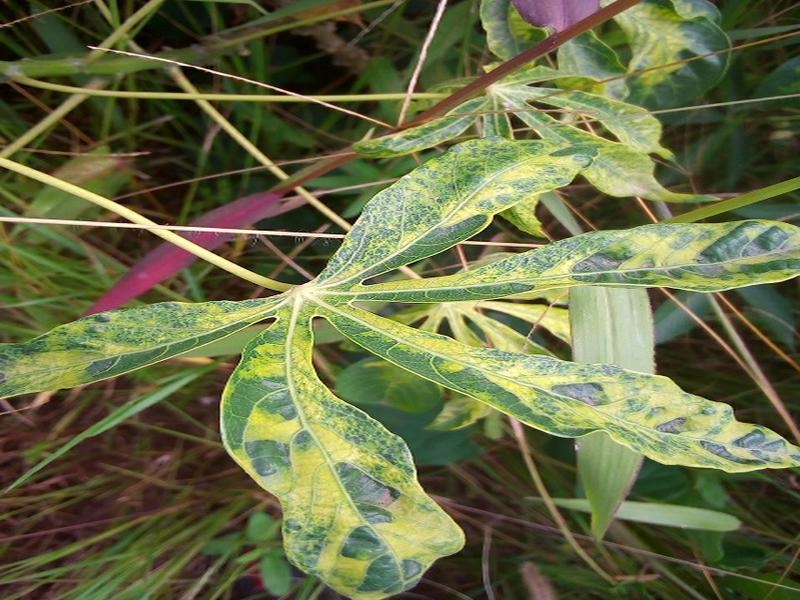
\includegraphics[width=\linewidth]{graphs/DiseaseImage/Mosaic.jpg}
        \caption{Mosaic}
        \label{CassavaFigMos}
    \end{subfigure}
    \caption{Cassava Disease Type}
    \label{CassavaDisease}
\end{figure}

The task aims to classify cassava leaf images based on the input data, to determine whether the leaf is healthy or infected by a specific type of virus illustrated before. Specifically, the input consists of image data with a resolution of $800 \times 600$ pixels, and the output is a category label indicating the leaf's condition. We categorize diseases from types $0$ to $3$ as Bacterial Blight through Mosaic and use category $4$ to label healthy cassava leaf images.

There are several challenges in the task. First, the original dataset has a significant class imbalance, with many more samples available for the Mosaic disease type than for the others. This imbalance can lead to biased model predictions, where the classifier favors the majority classes and underperforms the minority classes. Second, our analysis shows that a single model struggles to accurately capture and differentiate the characteristics of all virus types due to subtle visual differences among some categories. To address these challenges and improve overall classification performance, it is necessary to use strategies such as data augmentation, re-sampling techniques, and model fusion.

Our dataset comes from the public dataset on Kaggles~\cite{cassava-leaf-disease-classification}, which includes $21367$ labeled images during routine surveys conducted in Uganda. These images were captured by the farmers in their cassava gardens, which show real-world scenarios to distinguish different kinds of diseases.
